\section{Resultados}
\label{sec:4}

\subsection{Efecto de puertas en andén con demarcación}
\label{sec:4.1}
La \reffigura{fig4}{Ilustración 4} muestra la aplicación del modelo conceptual aplicado a las estaciones Ñuñoa y Ñuble. Se contó el número de veces que cada celda fue usada en pasajeros que esperan subir el tren durante la hora punta observada. En promedio de los 3 días observados se puede apreciar que el caso donde las puertas en andén poseen demarcación en el andén (Ñuble) una menor cantidad de pasajeros esperan al frente de las puertas en comparación con el caso sin demarcación (Ñuñoa). 

\begin{figure}
    \centering
    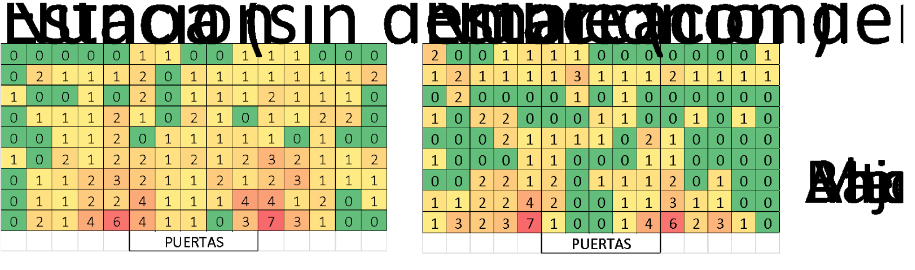
\includegraphics[width=0.8\textwidth]{imagenes/ilustracion_5.png}
    \caption{Número de veces en promedio que se usó cada celda cuando las puertas en anden no tienen demarcación (izquierda) y con demarcación (derecha) en las estaciones de Metro de Santiago}\label{fig5}
\end{figure}

Como consecuencia esto tiene un efecto en el número de filas de flujo de salida para pasajeros que bajan del tren. En el caso de Ñuble como hay menos pasajeros esperando frente a las puertas, se observó que los pasajeros que bajan del tren logran formar entre 1 y 2 filas de flujo. Sin embargo, en el caso de Ñuñoa solo se forma una sola fila de flujo para salir del tren. En términos de tiempo, el tiempo de bajada promedio por pasajero en Ñuble es de 0,88 s/pax, mientras que en el caso de Ñuñoa es de 0,92 s/pax, es decir un 4\% más.


\subsection{Efecto de puertas en andén con demarcación}
\label{sec:4.2}

Las 8 variables descritas en la Tabla 1 fueron observadas en la interfaz tren-andén de la Línea 1. Los resultados obtenidos muestran que un 96\% de las estaciones cuenta con ascensores, pues al momento del estudio solo Estación Central aún no poseía este elemento, el cual ya se encuentra en fase constructiva o finalizada junto con mejoras adicionales a la estación en accesos y pasillo de tránsito adicional para mejorar desplazamientos. Además, un 100\% posee asientos en andén, ancho de andén mayor a 3,0 m, intercomunicador a una altura menor a 1,2 m, y distancia entre el borde de andén y la línea amarilla mayor a 0,8 m. 

Si bien la interfaz tren-andén de la Línea 1 cumple con 6 de las 8 variables definidas en la Tabla 1, existe una variabilidad en el espesor de la línea amarilla e incluso esta no posee banda táctil (ver Ilustración 5). Asimismo, no todas las estaciones poseen pavimento guía y alerta (ver Ilustración 6). En resumen, solo 33\% de las estaciones cumplen el estándar de línea amarilla, según lo considerado en la Tabla 1, y 15\% poseen pavimento guía y alerta. 

Como consecuencia, y aplicando la métrica de accesibilidad en base a porcentajes equitativos por cada variable. Se puede observar en la Ilustración 7 que las estaciones menos accesibles son U.L.A. y República, mientras que la más accesible es Manquehue, llegando a un 100\% de cumplimiento en accesibilidad. Con esto, solo 9 estaciones (es decir un 33\%) cumplirían el mínimo porcentaje de accesibilidad definido como 70\% según el servicio SENADIS (Amestoy, 2015).



\begin{figure}
    \centering
    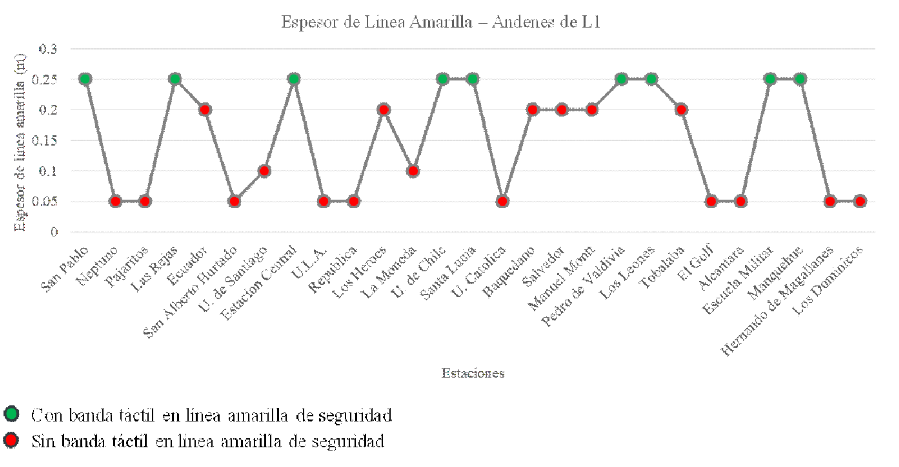
\includegraphics[width=0.8\textwidth]{imagenes/ilustracion_6.png}
    \caption{Accesibilidad estaciones con respecto al espesor de la línea amarilla y su uso con banda táctil en la interfaz tren-andén}\label{fig6}
\end{figure}

\begin{figure}
    \centering
    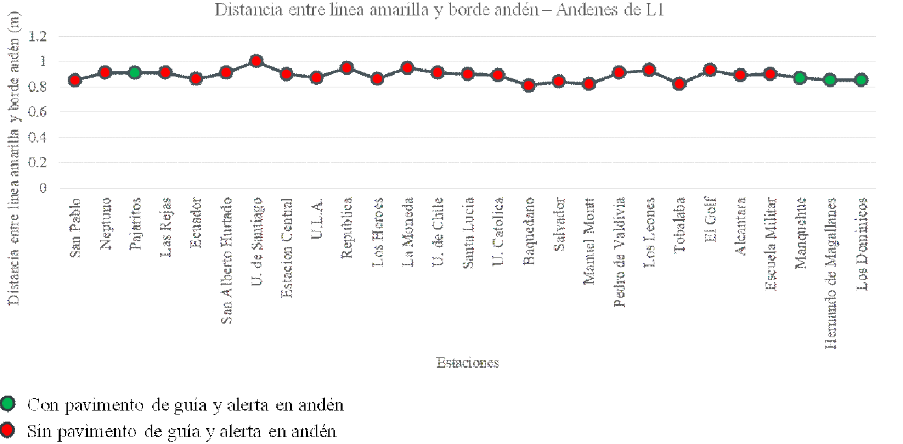
\includegraphics[width=0.8\textwidth]{imagenes/ilustracion_7.png}
    \caption{Accesibilidad estaciones respecto a la distancia entre el borde de anden y la línea amarilla junto con el uso de pavimento guía y alerta en la interfaz tren-andén}\label{fig7}
\end{figure}

\begin{figure}
    \centering
    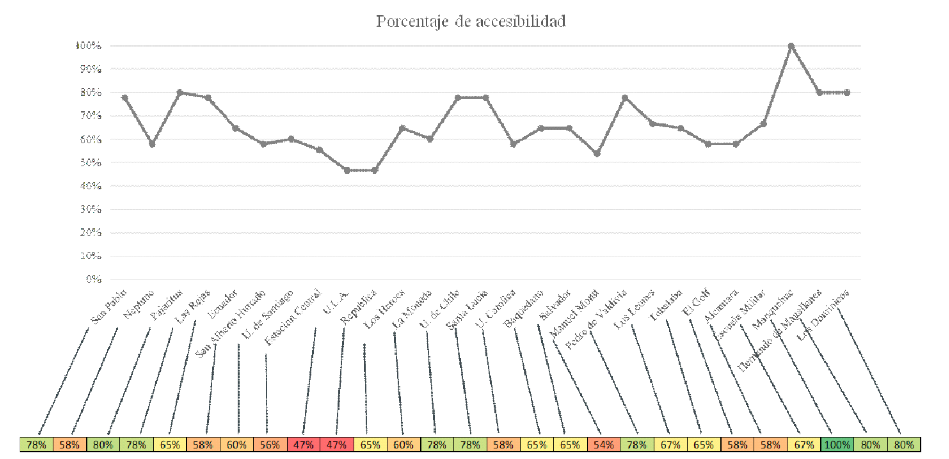
\includegraphics[width=0.8\textwidth]{imagenes/ilustracion_8.png}
    \caption{Porcentaje de accesibilidad total en la interfaz tren-andén en estaciones de la Línea 1}\label{fig9}
\end{figure}

\subsection{Experimentos en el Laboratorio de Dinámica Humana (LDH)}
\label{sec4.3}
De los resultados en la Tabla 3, se puede apreciar que la línea amarilla que más es respetada por parte de los participantes del experimento en el LDH es la de 40 cm, obteniendo un puntaje de 4,7. Luego la sigue la línea de 10 cm con un puntaje de 4,2. Con un puntaje similar le sigue la línea de 24 cm, con un puntaje de 4,1. Finalmente, la línea menos respetada por los pasajeros es la línea de 5 cm, con un puntaje de 3,7.
